 \documentclass[11pt]{article}
\def\shownotes{1}

\usepackage[top=3cm, bottom=3cm, left=2cm, right=2cm]{geometry}      % [top=2cm, bottom=2cm, left=2cm, right=2cm]
\geometry{letterpaper}                   % ... or a4paper or a5paper or ...
%\geometry{landscape}                % Activate for for rotated page geometry
%\usepackage[parfill]{parskip}
\usepackage{graphicx}
\usepackage{amssymb, amsmath, amsfonts}
\usepackage{amsthm}
\usepackage{enumerate}
\usepackage{hyperref}
\usepackage{xspace}
\usepackage{graphicx}
\usepackage{latexsym}
\usepackage{color}
\usepackage{framed}
\usepackage{algpseudocode}

\mathchardef\mhyphen="2D

\newcommand{\secref}[1]{\mbox{Section~\ref{#1}}}
\newcommand{\subsecref}[1]{\mbox{Subsection~\ref{#1}}}
\newcommand{\apref}[1]{\mbox{Appendix~\ref{#1}}}
\newcommand{\thref}[1]{\mbox{Theorem~\ref{#1}}}
\newcommand{\exref}[1]{\mbox{Example~\ref{#1}}}
\newcommand{\defref}[1]{\mbox{Definition~\ref{#1}}}
\newcommand{\corref}[1]{\mbox{Corollary~\ref{#1}}}
\newcommand{\lemref}[1]{\mbox{Lemma~\ref{#1}}}
\newcommand{\assref}[1]{\mbox{Assumption~\ref{#1}}}
\newcommand{\probref}[1]{\mbox{Problem~\ref{#1}}}
\newcommand{\clref}[1]{\mbox{Claim~\ref{#1}}}
\newcommand{\propref}[1]{\mbox{Proposition~\ref{#1}}}
\newcommand{\remref}[1]{\mbox{Remark~\ref{#1}}}
\newcommand{\consref}[1]{\mbox{Construction~\ref{#1}}}
\newcommand{\figref}[1]{\mbox{Figure~\ref{#1}}}
\DeclareMathOperator*{\expe}{\mathbb{E}}
\DeclareMathOperator*{\var}{\text{Var}}


\newcommand{\class}[1]{{\ensuremath{\mathsf{#1}}}}
\newcommand{\gen}{\ensuremath{\class{Gen}}\xspace}
\newcommand{\rep}{\ensuremath{\class{Rep}}\xspace}
\newcommand{\sketch}{\ensuremath{\class{SS}}\xspace}
\newcommand{\rec}{\ensuremath{\class{Rec}}\xspace}
\newcommand{\enc}{\ensuremath{\class{Enc}}\xspace}
\newcommand{\dec}{\ensuremath{\class{Dec}}\xspace}
\newcommand{\prg}{\ensuremath{\class{prg}}\xspace}
\newcommand{\zo}{\ensuremath{\{0, 1\}}}
\newcommand{\vect}[1]{\ensuremath{\mathbf{#1}}}
\newcommand{\zq}{\ensuremath{\mathbb{Z}_q}}
\newcommand{\Fq}{\ensuremath{\mathbb{F}_q}}
\newcommand{\sample}{\ensuremath{\class{Sample}}\xspace}
\newcommand{\neigh}{\ensuremath{\class{Neigh}}\xspace}
\newcommand{\dis}{\ensuremath{\mathsf{dis}}}
\newcommand{\decode}{\ensuremath{\mathsf{Decode}}}
\newcommand{\guess}{\mathsf{guess}}


\newcommand{\A}{\mathcal{A}}


\newcommand{\metric}{\ensuremath{\mathtt{Metric}}\xspace}
\newcommand{\hill}{\ensuremath{\mathtt{HILL}}\xspace}
\newcommand{\hillrlx}{\ensuremath{\mathtt{HILL\mhyphen rlx}}\xspace}
\newcommand{\yao}{\ensuremath{\mathtt{Yao}}\xspace}
\newcommand{\unp}{\ensuremath{\mathtt{unp}}\xspace}
\newcommand{\unprlx}{\ensuremath{\mathtt{unp\mhyphen rlx}}\xspace}
\newcommand{\metricstar}{\ensuremath{\mathtt{Metric}^*}\xspace}
\newcommand{\metricd}{\ensuremath{\mathtt{Metric}^*\mathtt{-d}}\xspace}
\newcommand{\hillstar}{\ensuremath{\mathtt{HILL}^*}\xspace}
\newcommand{\hillprime}{\ensuremath{\mathtt{HILL'}}\xspace}
\newcommand{\metricprime}{\ensuremath{\mathtt{Metric'}}\xspace}
\newcommand{\metricprimestar}{\ensuremath{\mathtt{Metric'}^*}\xspace}
\newcommand{\hillprimestar}{\ensuremath{\mathtt{HILL'}^*}\xspace}
\newcommand{\poly}{\ensuremath{\mathtt{poly}}\xspace}
\newcommand{\rank}{\ensuremath{\mathtt{rank}}\xspace}
\newcommand{\ngl}{\ensuremath{\mathtt{ngl}}\xspace}
\newcommand{\Hoo}{\mathrm{H}_\infty}
\newcommand{\Hav}{\tilde{\mathrm{H}}_\infty}
\newcommand{\Hfuzz}{\mathrm{H}^{\mathtt{fuzz}}_{t,\infty}}
\newcommand{\Huse}{\mathrm{H}_{\mathtt{usable}}}
\newcommand{\Dom}{\mathsl{Dom}}
\newcommand{\Range}{\mathsl{Rng}}
\newcommand{\Keys}{\mathsl{Keys}}
\def\col{\mathrm{Col}}

\newcommand{\ddetbin}{\ensuremath{\mathcal{D}^{det,\{0,1\}}}}
\newcommand{\drandbin}{\ensuremath{\mathcal{D}^{rand,\{0,1\}}}}
\newcommand{\ddetrange}{\ensuremath{\mathcal{D}^{det,[0,1]}}}
\newcommand{\drandrange}{\ensuremath{\mathcal{D}^{rand,[0,1]}}}

\newcommand{\expinfo}{\ensuremath{\mathcal{E}}}
\newcommand{\ext}{\ensuremath{\mathtt{ext}}}
\newcommand{\cext}{\ensuremath{\mathtt{cext}}}
\newcommand{\rext}{\ensuremath{\mathtt{rext}}}
\newcommand{\cons}{\ensuremath{\mathtt{cons}}}
\newcommand{\decons}{\ensuremath{\mathtt{decons}}}


\newcommand{\lwe}{\class{LWE}}
\newcommand{\LWE}{\class{LWE}}
\newcommand{\distLWE}{\ensuremath{\class{dist\mbox{-}LWE}}}

\newtheorem{theorem}{Theorem}[section]
\newtheorem{lemma}[theorem]{Lemma}
\newtheorem{proposition}[theorem]{Proposition}
\newtheorem{corollary}[theorem]{Corollary}
\newtheorem{definition}[theorem]{Definition}
\newtheorem{assumption}[theorem]{Assumption}
\newtheorem{claim}[theorem]{Claim}
\newtheorem{problem}[theorem]{Problem}
\newtheorem{construction}[theorem]{Construction}

\newcounter{ctr}
\newcounter{savectr}
\newcounter{ectr}

\newenvironment{newitemize}{%
\begin{list}{\mbox{}\hspace{5pt}$\bullet$\hfill}{\labelwidth=15pt%
\labelsep=5pt \leftmargin=20pt \topsep=3pt%
\setlength{\listparindent}{\saveparindent}%
\setlength{\parsep}{\saveparskip}%
\setlength{\itemsep}{3pt} }}{\end{list}}


\newenvironment{newenum}{%
\begin{list}{{\rm (\arabic{ctr})}\hfill}{\usecounter{ctr} \labelwidth=17pt%
\labelsep=5pt \leftmargin=22pt \topsep=3pt%
\setlength{\listparindent}{\saveparindent}%
\setlength{\parsep}{\saveparskip}%
\setlength{\itemsep}{2pt} }}{\end{list}}

\newenvironment{tiret}{%
\begin{list}{\hspace{2pt}\rule[0.5ex]{6pt}{1pt}\hfill}{\labelwidth=15pt%
\labelsep=3pt \leftmargin=22pt \topsep=3pt%
\setlength{\listparindent}{\saveparindent}%
\setlength{\parsep}{\saveparskip}%
\setlength{\itemsep}{2pt}}}{\end{list}}


\newenvironment{blocklist}{\begin{list}{}{\labelwidth=0pt%
\labelsep=0pt \leftmargin=0pt \topsep=10pt%
\setlength{\listparindent}{\saveparindent}%
\setlength{\parsep}{\saveparskip}%
\setlength{\itemsep}{20pt}}}{\end{list}}

\newenvironment{blocklistindented}{\begin{list}{}{\labelwidth=0pt%
\labelsep=30pt \leftmargin=30pt\topsep=5pt%
\setlength{\listparindent}{\saveparindent}%
\setlength{\parsep}{\saveparskip}%
\setlength{\itemsep}{10pt}}}{\end{list}}

\newenvironment{onelist}{%
\begin{list}{{\rm (\arabic{ctr})}\hfill}{\usecounter{ctr} \labelwidth=18pt%
\labelsep=7pt \leftmargin=25pt \topsep=2pt%
\setlength{\listparindent}{\saveparindent}%
\setlength{\parsep}{\saveparskip}%
\setlength{\itemsep}{2pt} }}{\end{list}}

\newenvironment{twolist}{%
\begin{list}{{\rm (\arabic{ctr}.\arabic{ectr})}%
\hfill}{\usecounter{ectr} \labelwidth=26pt%
\labelsep=7pt \leftmargin=33pt \topsep=2pt%
\setlength{\listparindent}{\saveparindent}%
\setlength{\parsep}{\saveparskip}%
\setlength{\itemsep}{2pt} }}{\end{list}}

\newenvironment{centerlist}{%
\begin{list}{\mbox{}}{\labelwidth=0pt%
\labelsep=0pt \leftmargin=0pt \topsep=10pt%
\setlength{\listparindent}{\saveparindent}%
\setlength{\parsep}{\saveparskip}%
\setlength{\itemsep}{10pt} }}{\end{list}}

\newenvironment{newcenter}[1]{\begin{centerlist}\centering%
\item #1}{\end{centerlist}}

\newenvironment{codecenter}[1]{\begin{small}\begin{centerlist}\centering%
\item #1}{\end{centerlist}\end{small}}

\ifnum\shownotes=1
\newcommand{\authnote}[2]{{\textcolor{red}{\textsf{#1 notes: }\textcolor{blue}{ #2}}\marginpar{\textcolor{red}{\textbf{!!!!!}}}}}
\else
\newcommand{\authnote}[2]{}
\fi
\newcommand{\bnote}[1]{{\authnote{Ben}{#1}}}
\newcommand{\lnote}[1]{{\authnote{Leo}{#1}}}
\newcommand{\rnote}[1]{{\authnote{Ran}{#1}}}
\newcommand{\onote}[1]{{\authnote{Omer}{#1}}}

\newcommand{\ve}{\vect{e}}
\newcommand{\vm}{\vect{m}}
\newcommand{\vy}{\vect{y}}
\newcommand{\vE}{\vect{E}}
\newcommand{\vS}{\vect{S}}
\newcommand{\vA}{\vect{A}}
\newcommand{\vc}{\vect{c}}
\newcommand{\vW}{\vect{W}}
\newcommand{\vQ}{\vect{Q}}
\newcommand{\vR}{\vect{R}}
\newcommand{\vU}{\vect{U}}
\newcommand{\vT}{\vect{T}}
\newcommand{\vX}{\vect{X}}
\newcommand{\vB}{\vect{B}}
\newcommand{\vz}{\vect{z}}
\newcommand{\vd}{\vect{d}}
\newcommand{\vs}{\vect{s}}
\newcommand{\vx}{\vect{x}}
\newcommand{\va}{\vect{a}}
\newcommand{\vb}{\vect{b}}
\newcommand{\vgamma}{\mathbf{\Gamma}}
\newcommand{\vt}{\vect{t}}
\newcommand{\vu}{\vect{u}}
\newcommand{\vF}{\vect{F}}
\newcommand{\recout}{x}
\newcommand{\ignore}[1]{}
\newcommand{\M}{\mathcal{M}}
\newcommand{\Vol}{\mathsf{Vol}}

\newcommand{\Succ}{\mathsf{Succ}}
\newcommand{\Adv}{\mathbf{Adv}}
 \newcommand{\Exp}{\mathbf{Exp}}

\title{When are Fuzzy Extractors Possible?}
\author{Benjamin Fuller\footnote{Boston University and MIT Lincoln Laboratory. The Lincoln Laboratory portion of this
work was sponsored by the Department of the Air Force under Air Force
Contract
\#FA8721-05-C-0002.  Opinions,
interpretations, conclusions and recommendations are those of the author
and
are not necessarily endorsed by the United States Government.  Email: {\tt bfuller@cs.bu.edu}.}~~~~~~~~~~Leonid Reyzin\footnote{Boston University.  Email: {\tt reyzin@cs.bu.edu}.}~~~~~~~~~~Adam Smith\footnote{Pennsylvania State University. Work done in part while the author was at Boston University and Harvard University.  Email: {\tt asmith@psu.edu}.  }}

\begin{document}
\maketitle

\begin{abstract}
We characterize when deriving a stable key from a noisy source is possible.  We use the notation of fuzzy extractors introduced by Dodis et al. (Eurocrypt 2004).  The goal is to produce a strong $key$ from a $w$ drawn from a \emph{strong} distribution $W$ and to produce the same when given a nearby $w'$.  A fuzzy extractor is split into two algorithms $\gen$ which produces $key$ along with some helper information $p$ and $\rep$ which takes $w'$ and $p$ to reproduce $key$.  The key must remain strong in the presence of $p$.  The goal is to produce the correct key whenever $\dis(w, w')\le t$.

Ideally, key derivation should be possible whenever a negligible portion of $W$ lies within a ball~(arbitrarily centered) of radius $t$.  We call the maximum weight that lies within any ball of radius $t$ the fuzzy min-entropy of a distribution.  In interactive information-reconciliation, fuzzy min-entropy is both a necessary and sufficient condition for security.  

Current techniques for constructing fuzzy extractors lie far from this necessary condition.  We investigate whether this is inherent for both fuzzy extractors and secure sketches~(a one round information-reconciliation component).  Our results are centered on feasibility and our constructions and impossibility results are primarily information-theoretic.  We consider two types of fuzzy extractors and secure sketches.  The first we call \emph{distribution-aware}, the algorithms know the precise distribution they are trying to correct.  The second is \emph{distribution-oblivious} where $(\gen, \rep)$ must work for a family of distributions.

\textbf{Distribution-Aware} In the distribution-aware setting we show that whenever the fuzzy min-entropy is super-logarithmic, there exists a secure sketch and fuzzy extractor with super-logarithmic output entropy.  That is, fuzzy min-entropy is both a necessary and \emph{sufficient} condition for security in this setting.

\textbf{Distribution-Oblivious} The distribution-oblivious situation is more complicated.  Indeed, there is a significant difference between secure sketches and fuzzy extractors.  We show that there exist families of distributions where each distribution has fuzzy min-entropy such that any secure sketch is insecure.  However, it is possible to build a fuzzy extractor for these same family of distributions.
\end{abstract}

\section{Introduction}
Usually, authentication requires some high quality secret.  Traditionally, this secret is assumed to have high min-entropy.  However, many sources with sufficient entropy for authentication present an additional problem of noise.  That is, when the physical instantiation of the source is read multiple times, readings are close~(according to some metric) but not identical.  To use such sources in an authentication scheme it is often necessary to remove this noise and derive the same key from the initial and subsequent readings.

This problem was introduced in the seminal work of Bennett, Brassard, and Roberts~\cite{bennett1988privacy}.  They identify two fundamental tasks in noisy key derivation.  The first is known as information-reconciliation, removing the noise without leaking significant information, and the second is privacy amplification, converting the high entropy secret to a uniform random value.  In this work, we consider the non-interaction version of these problems where these tasks are performed non-interactively~(with a single message).

The paradigm for performing noisy key derivation using a single metric is known as fuzzy extractors~\cite{DBLP:journals/siamcomp/DodisORS08}.  Consider a particular high entropy distribution $W$.  Our goal is to derive stable keys from $W$ whenever the two readings~(denoted $w$ and $w'$ respectively) are within distance $t$.  A fuzzy extractor consists of two algorithms: generate~($\gen$) which takes the initial reading $w$ and produces $key$ along with a public helper value $p$.  The reproduce~($\rep$) algorithm takes the subsequent reading $w'$ along with the helper value $p$ to reproduce $key$.  The $key$ must be strong even to an adversary that has observed $p$~(the problem is trivial if $p$ is private).

Traditionally, fuzzy extractors are constructed by using a separate information-reconciliation component, known as a secure sketch, that maps $w'$ back to $w$ and a privacy-amplification component, a strong randomness extractor~\cite{nisan1993randomness}, that maps $w$ to a random key.  These objects can either be information-theoretic or computational.  The computational versions of these objects are defined in~\cite{krawczyk2010cryptographic} and~\cite{fuller2013computational} respectively.  Fuller et al.~\cite{fuller2013computational} show that computational secure sketches are unlikely to improve significantly on information-theoretic secure sketches.

\textbf{A Necessary Condition:}  Intuitively, error-tolerance and key strength are at odds.  If the error-tolerance allows the entire metric space to authenticate then no security is possible.  As an example, consider a distribution $W$, where the adversary attempts to learn the key simply by inputting a point to the reproduce function.  Let $x^*$ be the point input by the adversary, the adversary learns the correct key whenever $\dis(w, x^*)\le t$.  For a fuzzy extractor to be secure this must occur with negligible probability.  That is, a negligible portion of the probability mass of $W$ may be close to any point in the metric space.  Mathematically, for all $x^*, \sum_{w\in W | \dis(w, x^*)\le t} \Pr[ W= w] \le \ngl(n)$.  We call the negative logarithm of this quantity the \emph{fuzzy min-entropy} of a distribution.  The fuzzy min-entropy of a distribution must be super-logarithmic for any reasonable of either a fuzzy extractor~(\lemref{lem:fuzz necessary}).  

In the more general interactive setting where two parties hold $w$ and $w'$ and wish to agree on a common key, fuzzy min-entropy is both a necessary and sufficient condition~(using two-party computation). 
However, in the one-message setting we are far from achieving security whenever fuzzy min-entropy is high.


Traditional fuzzy extractors and secure sketches incur at entropy loss of the size of the ball to be error-corrected.  While, this is optimal for the uniform distribution, it is far from optimal for distributions that arise in practice.  As an example, many examples that arise in practice there are more error patterns than starting entropy.  Traditional fuzzy extractors provide no guarantee for sources of this type.  The work of Canetti et al.~\cite{canetti2014key} shows it is possible to provide build fuzzy extractors for some distributions with this property.  Their work leaves the question open for a large number of distributions.  This leads to the following natural question: \emph{when is key derivation from noisy sources possible?}

When building a fuzzy extractor, the algorithm designer has some information about the distribution $W$ that will be used.  However, rarely does the algorithm designer know the entire description of $W$'s probability distribution~(indeed this description may be exponential size).  This uncertainty is usually expressed by proving the fuzzy extractor works for a class of distributions with some known property~(such as entropy and error levels).  In this work, we discriminate between fuzzy extractors and secure sketches that are allowed to know the distribution of $W$ and algorithms that are required to work for a family of distributions $\mathcal{W}$.  We call the first type of algorithm \emph{distribution-aware} and the second type \emph{distribution-oblivious}

\textbf{Our Contribution} We show that for every distribution with super-logarithmic fuzzy min-entropy it is information-theoretically possible to build a secure sketch that retains super-logarithmic min-entropy.  Using standard techniques we can convert this secure sketch to a fuzzy extractor with super-logarithmic key output length.  (A key with super-logarithmic entropy can be expanded to arbitrary length using computational techniques.)  For distribution-aware secure sketches and fuzzy extractors, fuzzy min-entropy is both a necessary and sufficient condition for security.  

The situation is significantly more complicated for distribution-oblivious algorithms.  Indeed, we show that there natural families to distributions where every distribution has fuzzy min-entropy such that no secure sketch can provide meaningful security.  However, it is possible to build a meaningful fuzzy extractor for this same class of distributions.

\textbf{Note:} Our constructions are information-theoretic and do not run in polynomial time.  They should primarily be regarded as feasibility results.  Our negative results apply to algorithms even given arbitrary running time, thus there is clear separation for unbounded running time algorithms.  It remains as an open question whether our distribution-aware results can be replicated by efficient algorithms.  This seems unlikely as most  interesting distributions have exponential size description.  The power of the distribution-aware setting is that the algorithms can access this description.  It seems unlikely that algorithms with access to a polynomial size part of the distribution description can replicate these results.

\textbf{Open Problems:} We showed that in the distribution-oblivious setting there is a separation between a secure sketch and a fuzzy extractor.  However, it is still not known if fuzzy extractors can be constructed for any family of distributions.

\begin{table}
\begin{center}
\begin{tabular}{c | c | c }
& Distribution-Aware & Distribution-Oblivious\\
\hline
Secure Sketch & Yes~(\thref{cons:leveling}) & No\\
\hline
Fuzzy Extractor & Yes~(\thref{cons:leveling}) & Yes for some families\\
& & Unknown for arbitrary family
%Flat distribution & $\Hfuzz(W) - \log (1/\delta)$ &$\log |B_t|$\\
%Arbitrary distribution & $\Hfuzz(W) - \log (1/\delta) - \log \log \mathcal{M}$ & $\log |B_t|$
\end{tabular}
\end{center}
\caption{Is fuzzy min-entropy sufficient for extraction?}
\label{tab:main results}
\end{table}


\bnote{connection to obfuscation}
\section{Preliminaries}
\label{sec:preliminaries}
\bnote{be careful with overloading of $\ell$, both key length and number of levels.}
For a random variables $X_i$ over some alphabet $\mathcal{Z}$ we denote by $X = X_1,..., X_\ell$  the tuple $(X_1,\dots, X_\ell)$.  For a set of indices $J$, $X_{J}$ is the restriction of $X$ to the indices in $J$.  The set $J^c$ is the complement of $J$.  The {\em min-entropy} of $X$ is $\Hoo(X) = -\log(\max_x \Pr[X=x])$,
and the {\em average (conditional)} min-entropy of $X$ given $Y$ is  $\Hav(X|Y) = -\log(\expe_{y\in Y} \max_{x} \Pr[X=x|Y=y])$~\cite[Section 2.4]{DBLP:journals/siamcomp/DodisORS08}.   For a random variable $W$, let $H_0(W)$ be the logarithm of the size of the support of $W$,  that is $H_0(W) = \log |\{w | \Pr[W=w]>0\}|$.  We will also use an average case version of this notion~(to the best of our understanding this has not been used before):\bnote{has it?}
\begin{definition}[Conditional Hartley Entropy]
\label{def:conditional hartley}
The conditional Hartley entropy of $X |Y $ is $\tilde{H}_0(X |Y) = \log ( \expe_{y\in Y} |\{x | \Pr[X=x |Y=y]>0\}|)$.
\end{definition}
The {\em statistical distance} between random variables $X$ and $Y$ with the same domain is $\Delta(X,Y) = \frac12 \sum_x |\Pr[X=x] - \Pr[Y=x]|$.
For a distinguisher $D$ we write the \emph{computational distance} between $X$ and $Y$ as $\delta^D(X,Y) = \left| \expe[D(X)]-\expe[D(Y)]\right |$ (we extend it to a class of distinguishers $\mathcal{D}$ by taking the maximum over all distinguishers $D\in\mathcal{D}$).  We denote by $\mathcal{D}_{s}$ the class of randomized circuits which output a single bit and have size at most $s$.

For a metric space $(\mathcal{M}, \dis)$, the \emph{(closed) ball of radius $t$ around $x$} is the set of all points within radius $t$, that is, $B_t(x) = \{y| \dis(x, y)\leq t\}$.  If the size of a ball in a metric space does not depend on $x$, we denote by $|B_t|$ the size of a ball of radius $t$.  We consider the Hamming metric over vectors in $\mathcal{Z}^\ell$, defined via $\dis(x,y) = \{i | x_i \neq y_i\}$.  For this metric, $|B_t| = \sum_{i=0}^t {\ell \choose i} (|\mathcal{Z}|-1)^i $.  $U_n$ denotes the uniformly  distributed random variable on $\{0,1\}^n$.  Unless otherwise noted logarithms are base $2$.
Usually, we use capitalized letters for random variables and corresponding lowercase letters for their samples.

\section{Fuzzy Extractors}\label{sec:fuzz extractor}

We now recall definitions and lemmas from the work of Dodis et. al.~\cite[Sections 2.5--4.1]{DBLP:journals/siamcomp/DodisORS08}, adapted to allow for a small probability of error, as discussed in \cite[Sections 8]{DBLP:journals/siamcomp/DodisORS08}.  Let $\mathcal{M}$ be a metric space with distance function $\dis$.

\begin{definition}
\label{def:fuzzy extractor}
An $(\mathcal{M}, m, \ell, t, \epsilon)$-\emph{fuzzy extractor} with error $\delta$ is a pair of randomized procedures, ``generate'' $(\gen)$ and ``reproduce'' $(\rep)$, with the following properties: 
\begin{enumerate}
\item The generate procedure \gen on input $w\in \mathcal{M}$ outputs an extracted string $r\in\{0,1\}^\ell$ and a helper string $p\in\{0,1\}^*$.
\item The reproduction procedure \rep takes an element $w'\in \mathcal{M}$ and a bit string $p\in\{0,1\}^*$ as inputs.  The \emph{correctness} property of fuzzy extractors guarantees that for $w$ and $w'$ such that $\dis(w,w')\leq t$, if $R,P$ were generated by $(R,P)\leftarrow\gen(w)$, then $\rep(w',P)=R$ with probability~(over the coins of $\gen, \rep$) at least $1-\delta$.  If $\dis(w,w')>t$, then no guarantee is provided about the output of \rep.
\item The \emph{security} property guarantees that for any distribution $W$ on $\mathcal{M}$ of min-entropy $m$, the string $R$ is nearly uniform even for those who observe $P$:  if $(R,P)\leftarrow\gen (W)$, then $\mathbf{SD}((R,P),(U_\ell,P))\leq \epsilon$.
\end{enumerate}
A fuzzy extractor is efficient if $\gen$ and $\rep$ run in expected polynomial time.
\end{definition}

Replacing the statistical distance in \defref{def:fuzzy extractor} with computational distance results in a \emph{computational fuzzy extractor}~\cite[Definition 2.5]{fuller2013computational}.  A fuzzy extractor performs two tasks, producing a uniform key and providing error-tolerance.  Traditional, the uniform key is produced by extraction from the original secret $w$ and the error-tolerance is obtained by using a secure sketch.  Secure sketches produce a string $s$ that does not decrease the entropy of $w$ too much, while allowing recovery of $w$ from a  close $w'$:
\begin{definition}
\label{def:secure sketch}
An $(\mathcal{M},m, \tilde{m}, t)$-\emph{secure sketch} with error $\delta$ is a pair of randomized procedures, ``sketch'' $(\sketch)$ and ``recover'' $(\rec)$, with the following properties:
\begin{enumerate}
\item The sketching procedure \sketch on input $w\in\mathcal{M}$ returns a bit string $s\in\{0,1\}^*$.
\item The recovery procedure \rec takes an element $w'\in\mathcal{M}$ and a bit string $s\in\{0,1\}^*$.  The \emph{correctness} property of secure sketches guarantees that if $\dis(w,w')\leq t$, then $\Pr[\rec(w',\sketch(w))=w]\geq 1-\delta$ where the probability is taken over the coins of $\sketch$ and $\rec$.  If $\dis(w,w')>t$, then no guarantee is provided about the output of \rec.
\item The \emph{security} property guarantees that for any distribution $W$ over $\mathcal{M}$ with min-entropy $m$, the value of $W$ can be recovered by the adversary who observes $w$ with probability no greater than $2^{-\tilde{m}}$.  That is, $\Hav(W|\sketch(W))\geq \tilde{m}$.
\end{enumerate}
A secure sketch is \emph{efficient} if \sketch and \rec run in expected polynomial time. 
\end{definition}

\textbf{Notes:} In the above definition of secure sketches (resp., fuzzy extractors), the errors are chosen before $s$ (resp., $P$) is known: if the error pattern between $w$ and $w'$ depends on the output of $\sketch$ (resp., $\gen$), then there is no guarantee about the probability of correctness.  We do not consider a computational version of secure sketches. Fuller et al. showed that computational secure sketches imply information-theoretic secure sketches with almost the same parameters~\cite[Corollary 3.8]{fuller2013computational}.


A fuzzy extractor can be produced from a \emph{secure sketch} and an \emph{average-case randomness extractor}. An average-case extractor is a generalization of a strong randomness extractor \cite[Definition 2]{nisan1993randomness}) (in particular, Vadhan~\cite[Problem 6.8]{Vad12} showed that all strong extractors are average-case extractors with a slight loss of parameters):
\begin{definition}
Let $\chi_1$, $\chi_2$ be finite sets.
A function $\ext: \chi_1\times \{0,1\}^d \rightarrow \{0,1\}^\ell$ a \emph{$(m, \epsilon)$-average-case extractor} if for all pairs
of random variables $X, Y$ over $\chi_1, \chi_2$ such that
$\tilde{H}_\infty(X|Y) \ge m$, we have $\Delta((\ext(X, U_d), U_d, Y), U_\ell\times
U_d \times Y) \le \epsilon$.
\end{definition}

\begin{lemma}
\label{lem:fuzzy ext construction}
Assume $(\sketch, \rec)$ is an $(\mathcal{M}, m, \tilde{m}, t)$-secure sketch with error $\delta$, and let $\ext:\mathcal{M}\times \zo^d \rightarrow \zo^\ell$ be a $(\tilde{m}, \epsilon)$-average-case extractor.  Then the following $(\gen, \rep)$ is an $(\mathcal{M}, m, \ell, t, \epsilon)$-fuzzy extractor with error $\delta$:
\begin{itemize}
\item $\gen(w):$ generate $x\leftarrow \zo^d$, set $p=(\sketch(w), x), r=\ext(w;x)$, and output $(r,p)$.
\item $\rep(w', (s, x)):$ recover $w=\rec(w',s)$ and output $r=\ext(w;x)$.
\end{itemize}
\end{lemma}

\subsection{A necessary condition for security}
\label{sec:minimal conditions}
Consider the functionality of a fuzzy extractor, the reproduce algorithm produces the same key when provided with a nearby input point.  In an ideal world, this would be all that is revealed by the reproduce algorithm.  For the remainder of this work, we compare security with this ideal world.  This ideal world can be expressed by an adversary providing a ``guess'' point to the algorithm~(and hoping that their guess was closed to the stored point).  We call the level of security in this setting, fuzzy min-entropy.
%\todo{doesn't 2PC require assumptions?}
%We now define fuzzy min-entropy and show that fuzzy extractor security is only possible when the fuzzy min-entropy is super-logarithmic.

%A necessary condition for fuzzy extractor security is that an adversary should not be able to learn the key simply by inputting a point into the \rep algorithm.  This means a negligible portion of the source distribution $W$ lies within any Hamming ball.  We make this intuition formal here:

\begin{definition}
\label{def:fuzzy min-ent}
A distribution $W$ in a metric space $(\mathcal{M}, \dis)$ has $(t, k)$-fuzzy min-entropy, denoted $\Hfuzz(W) \ge k$ if the following holds:
\[
\forall m\in \mathcal{M},  \sum_{w\in W | \dis(w, m)\le t} \Pr[W=w] \leq 2^{-k}.
\]
\end{definition}

If an adversary can always obtain the output of a fuzzy extractor by running the reproduce adversary, then there is no hope for security~(independent of the implementation of the fuzzy extractor).  We make this intuition formal in the following result.  
For a metric space $\mathcal{M}$, let $\max |\mathcal{M}|$ the maximum length required to describe an element $m\in\mathcal{M}$~(for most natural metric spaces this is $\log |\mathcal{M}|$).
\begin{lemma}
\label{lem:fuzz necessary}
Let $n$ be a security parameter and let $W$ be a distribution over $(\mathcal{M}, \dis)$.
If $\Hfuzz (W) = \Theta(\log n)$ there is no $(\mathcal{M}, W, \kappa, t)$-computational fuzzy extractor that is $(\max |\mathcal{M}| +  |\rep|, \epsilon)$-hard for $\epsilon = \ngl(n)$ with error $\delta = \ngl(n)$~(and thus no fuzzy extractor) for $\kappa =\omega(\log n)$.
\end{lemma}
\begin{proof}
Let $W$ be a distribution where $\Hfuzz(W) = \Theta(\log n)$.  This means that there exists a point $m^*\in \mathcal{M}$ such that $\Pr_{w\in W}[\dis (w, m^*)\leq t] \geq 1/\poly(n)$.  Consider the following distinguisher $D$:
\begin{itemize}
\item Input $r, p$.
\item If $\rep(m^*, p) = r$, output $1$.
\item Else output $0$.
\end{itemize}
First note that $|D|$ is of size $\max |\mathcal{M}|+ |\rep|$.  Clearly, $\Pr[D(R, P) = 1]\geq 1/\poly(n) - \delta$, while $\Pr[D(U_\kappa, P)=1 ]= 1/2^{-\kappa}$.  Thus, when $\kappa = \omega(\log n)$:
\[
\delta^D((R, P), (U_\kappa, P))\geq \frac{1}{\poly(n)} -\delta -  \frac{1}{2^{-\kappa}} = 1/\poly(n).
\]
\end{proof}
\lemref{lem:fuzz necessary} generalizes to interactive protocols, $D$ only provides an input to the protocol and looks at the output.  This means that fuzzy min-entropy is also a necessary condition for interactive solution.  As stated above, fuzzy min-entropy is also a sufficient condition for security in the interactive setting.  However, in the fuzzy extractor~(non-interactive) setting there are many distributions for which no construction is known to be secure and for which no impossibility result is known.  We attempt to bridge this gap in this work.  

Before turning to our results we separate between two types of fuzzy extractors and secure sketches.  The standard definition requires a fuzzy extractor/secure sketch to work for a family of distributions.  We call this type of algorithm distribution-oblivious.  We define a new type of algorithm that called distribution-aware that is allowed to know the precise distribution to be supported.  We provide a definition for secure sketches~(this definition can easily be extended to fuzzy extractors)

\begin{definition}
Let $W$ denote a distribution.  A secure sketch, $(\sketch_W, \rec_W)$ is called \emph{distribution-aware} if the correctness and security properties hold for the distribution $W$.  That is, 
\begin{enumerate}
\item \emph{Correctness} For all $w\in W$ and for all $w'\in\mathcal{M}$,  if $\dis(w,w')\leq t$, then $\Pr[\rec(w',\sketch(w))=w]\geq 1-\delta$ where the probability is taken over the coins of $\sketch$ and $\rec$.  If $\dis(w,w')>t$, then no guarantee is provided about the output of \rec.  Note correctness is guaranteed only for the support of $W$.
\item \emph{Security} The distribution $W$ is unknown conditioned on $s$: $\Hav(W|\sketch(W))\geq \tilde{m}$.
\end{enumerate}
\end{definition}
Note that correctness is only required to hold for points in the support of the distribution $W$, the algorithms are allowed the description of $W$ and security need only hold for the distribution $W$.  When we consider distribution-aware algorithms, we generally assume they are \emph{inefficient}, this seems inherent to make use of the (possibly)~exponential size distributions.  It is not clear how to meaningfully define efficient distribution aware algorithms.  If the algorithms were required to be efficient, they could only encode a negligible portion of the probability space of $W$, and would have to ``work'' on all distributions $W'$ with the same probability mass function on the encoded space.  This would make the algorithms a distribution-oblivious fuzzy extractor for all distributions with this property.

We begin with by showing that secure sketches and fuzzy extractors are possible in the distribution aware setting whenever there is super-logarithmic fuzzy min-entropy.  We then turn to the standard \emph{distribution oblivious} setting.

%The summary of our results is in Table~\ref{tab:upper bounds}.

\begin{table}
\begin{tabular}{l | l | c}
Lower bounds & Distribution-Dependent & Distribution-Oblivious\\
\hline
Well-spread distribution & $\Hfuzz(W)$ & $\log |B_t|$\\
Flat distribution & $\Hfuzz(W) - \log (1/\delta)$ &$\log |B_t|$\\
Arbitrary distribution & $\Hfuzz(W) - \log (1/\delta) - \log \log \mathcal{M}- O(1)$ & $\log |B_t|$
\end{tabular}
\caption{Residual entropy of secure sketches for complete recovery.}
\label{tab:upper bounds}
\end{table}
\bnote{Fix right side of table}
\bnote{the table should move.}
%We begin with the left column of Table~\ref{tab:upper bounds} and provide constructions of sketches~(which generalize to fuzzy extractors).  We then show that building distribution-agnostic secure sketches and fuzzy extractors is significantly harder.

\section{Distribution-Aware  Sketches}
In this section, we consider show it is possible to build distribution-aware fuzzy extractors and secure sketches whenever $\Hfuzz(W)= \omega(\log n)$.
We consider increasingly complex types of distributions and end with an arbitrary distribution over a metric space.  We construct secure sketches but our constructions can be transformed to fuzzy extractors using \lemref{lem:fuzzy ext construction}.  In \secref{sec:dist oblivious} we consider distribution-oblivious algorithms.  

\subsection{Well-Spread Distributions}
We call a distribution well-spread if the distance between any two original readings $w_0, w_1$ is large.  Well-spread distributions should be the easiest type of distribution to handle as given a particular $w'$ there is a unique $w$ that could be the original reading.  Error-correction is ``easy'' when all points of $W$ are far apart.  Intuitively, the fuzzy extractor/secure sketch does not need to disambiguate points.  %Indeed for any error-correcting code, a fuzzy extractor can be designed~(where the design of the fuzzy extractor depends on the supported distribution).  However, this intuition becomes more difficult when a fuzzy extractor should work for all well-spread distributions.  
We begin by defining a well-spread distribution.

\begin{definition}
A distribution $W$ is called \emph{$t_{cor}$-well spread} if for all $w, x\in W, \dis(w, x)\ge t_{cor}$.
\end{definition}
Intuitively, it should be easy to build a fuzzy extractor for well-spread distributions when the desired error-tolerance is less than $t_{cor}/2$~(assuming the distribution has super-logarithmic min-entropy).  Indeed, this is the case when the fuzzy extractor is allowed to depend on $W$.\footnote{This result can be viewed as saying that well-spread distributions are not interesting in the distribution-aware setting.  However, we will show that providing secure sketches for well-spread distributions in the distribution-oblivious setting is impossible.}

\begin{lemma}
\label{lem:nosketchwellspread}
Let $W$ be a $t_{cor}$ well-spread distribution with $\Hoo(W)\ge k$ there exists a $(\mathcal{M}, m, m, \lfloor( t_{cor}-1)/2\rfloor)$-secure sketch with no error that works for $W$.  In particular, $\sketch(w) = \perp$, and $\rec(w')$ finds the nearest $w\in W$.  \rec is efficient if there exists efficient decoding for the points in $W$.  By \lemref{lem:fuzzy ext construction} there also exists a $(\mathcal{M}, m,m -2\log 1/\epsilon, \lfloor (t_{cor}-1)/2\rfloor, \epsilon)$-fuzzy extractor with no error.
\end{lemma}  
\begin{proof}
It suffices to show that for any $w'$ there exists a unique $w\in W$ such that $\dis (w, w')\le \lfloor (t_{cor}-1)/2\rfloor$.  Since $W$ is $t_{cor}$-well spread, for all $w_0, w_1 \in W, \dis (w_0, w_1)\ge t_{cor}$.  Then by the triangle inequality,
\[
t_{cor}\ge \dis(w_0, w_1) \ge \dis(w_0, w') + \dis(w', w_1).\]
This is only true if at least one of $\dis(w_0, w')$ or $\dis(w', w_1)$ is greater than $\lfloor (t_{cor}-1)/2\rfloor$.
\end{proof}

\subsection{Flat distributions}
In the previous section we showed it is easy to produce secure sketch for well-spread distributions in the distribution aware setting.
%\lemref{lem:nosketchwellspread} showed that if a fuzzy extractor~(resp. secure sketch) is built for a particular well-spread distribution, it is not necessary to write down information-reconciliation information.  
In this section, we consider distributions with multiple points in each ball where points have the same probability.

\begin{definition}
A distribution $W$ is \emph{flat} if for all $w_0, w_1 \in W$, $\Pr[W=w_0] = \Pr[W=w_1]$.  
\end{definition}

Recall that fuzzy min-entropy is a lower bound of the adversaries success probability for any scheme.  Fuzzy min-entropy is total weight of the maximum probability ball~(\defref{def:fuzzy min-ent}).  For flat distributions, this is proportional to the largest number of points in any ball.  More precisely, 
\begin{align*}
\Hfuzz(W) &= -\log \left(\max_{w^* \in \mathcal{M}} \left| \{w | w\in W \wedge \dis(w, w^*)\le t\} \right|* \Pr[W=w]\right) \\
&= -\log\left( \max_{w^* \in \mathcal{M}} |\{w | w\in W \wedge \dis(w, w^*)\le t\}| *2^{-\Hoo(W)}\right) \\
&=\Hoo(W) -\log\left( \max_{w^* \in \mathcal{M}}| \{w | w\in W \wedge \dis(w, w^*)\le t\} |\right)
\end{align*}
For notational convenience, we denote the ball with the largest number of points as $B_{t, max}$.  For any scheme, the adversary's success probability is 
\begin{align}
\Hfuzz(W) = \Hoo(W) -\log |B_{t, max}|.\label{eq:fuzz for flat}
\end{align}
%We start by considering distributions that have a fixed number of neighbors for each point.
%
%\begin{definition}
%We call a distribution $W$, over metric space $\mathcal{M}$, $(c, t)$-\emph{fixed neighbor} if there exists a constant $c$ such that for all points in $x\in \mathcal{M}$ there are exactly $c$ points $w\in W$ such that $\dis(w, x)\le t$.  We say that $W$ is a $(c, t)$-\emph{bounded neighbor distribution} if for all point $x\in\mathcal{M}$ there are at most $c$ points $w\in W$ such that $\dis(w, x)\le t$.
%\end{definition}
%
%\textbf{Note:} A fixed neighbor distribution is a special case of a bounded-neighbor distribution.
We now present a construction for flat distributions.  We use pairwise-independent hashes:

\begin{definition}
Let $F : \mathcal{K} \times D \to R$ be a function.  We say that $F$ is \emph{universal} if for all distinct $x_1, x_2 \in D$:
\[
 \Pr_{K \leftarrow \mathcal{K}}[F(K, x_1) = F(K, x_2)] = \frac{1}{|R|} \;.
\]
%In other words, $F(K,x_1),F(K,x_2)$ are all uniformly and independently random over $R$. 
\end{definition}

We now show a sufficiently-long universal hash function suffices to construct an information-theoretic fuzzy extractor.  The work of Skoric et al.~\cite{skoric2009efficient} use universal hash functions in the setting where there are a polynomial number of possible error patterns.

\begin{construction}
\label{cons:pairwise hash}
Let $W$ be a flat distribution over $\mathcal{M}$.  Let $F :\mathcal{K}\times \mathcal{M}\rightarrow R$ be a pairwise independent hash function.  We describe $\sketch, \rec$ as follows:
\begin{itemize}
\item $\sketch(w)$:
\subitem Sample $K\leftarrow \mathcal{K}$.
\subitem Set $p = F(K, w), K$.
\item $\rec(w', y, K)$:
\subitem Enumerate $W^* = \{w \in W | \dis(w, w')\le t\}$.
\subitem For all $w^*\in W^*$, if $F(K, w^*) = y$, output $w^*$.
\subitem Output $\perp$.
\end{itemize}
\end{construction}
\begin{lemma}
\consref{cons:pairwise hash} is a $(\mathcal{M}, m, m - \log |R|, t)$-secure sketch with error $\delta \le \frac{|B_{t, max}|-1}{|R|}$. 
\end{lemma}
\begin{proof}
We first argue security.  Since $\mathcal{K}$ and $W$ are independent $\Hav(W | \mathcal{K}) = \Hoo(W) = m$.  Then by \cite[Lemma 2.2b]{DBLP:journals/siamcomp/DodisORS08}, $\Hav(W | \mathcal{K}, F(K, W)) \ge \Hoo(W) - \log |F(K, W)| \ge m - \log |R|$.

We now argue correctness.  Fix some $w, w'$.  Let $W^*$ denote the set of elements in $W$ within distance $t$ of $w'$ recall that the size of $W^*$ is at most $B_{t, max}$ and since $w, w'$ are chosen independently of $\sketch$ this set is independent of the choice of $\mathcal{K}$.  Note $\rec$ will never output $\perp$ as the correct $w$ will match the hash, our goal is to bound the probability that another element $w^*$ collides, that is $F(K, w^*) = F(K, w)$.
\begin{align*}
\Pr[\exists w^* \in W^* |w^* \neq w \wedge F(K, w^*) = F(K, w)] &\le \sum_{w^*\in W^* | w^*\neq w} \Pr[F(K, w^*) = F(K, w)] \\
 &= \sum_{w^*\in W^* | w^*\neq w} \frac{1}{|R|} \le \frac{|B_{t, max}|-1}{|R|}
\end{align*}
Where the inequality proceeds by union bound, the first equality proceeds by the universality of $F$, and the second inequality proceeds by noting the number of neighbors is bounded by $|B_{t, max}|-1$.  This completes the proof.
\end{proof}
\begin{corollary}
Let $n$ be a security parameter.  
If $|R| \ge |B_{t, max}|* n^{\omega(1)}$ then \consref{cons:pairwise hash} is correct with overwhelming probability.  That is, setting $\log |R| = \log |B_{t, max}| + \omega(\log n)$ suffices.
\end{corollary}

Note that \consref{cons:pairwise hash} writes down essentially the worst case number of bits in all setting, it knows the maximum number of points in any ball and writes down that number~(with an additional super-logarithmic factor to prevent collisions).  Recall, our hope is to find a sketch that achieves total security equal to the fuzzy min-entropy of the distribution.  Thus, the remaining entropy for this construction is 
\[
\Hav(W |\sketch(W)) = \Hoo(W) - \log |B_{t, max}| - \omega(\log n)
\]
For a flat distribution this is within a super-logarithmic factor of optimal~(see Equation~\eqref{eq:fuzz for flat}).  Furthermore, whenever $\Hfuzz(W) = \omega(\log n)$, we can construct a secure sketch that is correct with overwhelming probability while retaining a super-logarithmic amount of entropy~(by choosing $\delta$ depending on $\Hfuzz(W)$).  That is, we can construct a secure sketch whenever there is super-logarithmic starting entropy.  Intuitively, this is because the sketch is deconflicting for the ball with the largest number of points.  For a flat distribution, this is also the ball with the largest total weight.  We will see this becomes more difficult as we move to the setting where points have very different probability.  %In this setting, we may write down a large number of bits to deal with a low weight ball that has a large number of points, but this may completely reveal the high weight balls. We will compensate for this problem by writing down a variable number of bits.
%with a fixed number of neighbors, 
%\begin{align*}
%\Hfuzz(W) &= -\log \max_{x\in \mathcal{M}}, \sum_{w | \dis(w, x)\le t} \Pr[W=w]\\
%&=-\log \max_{x\in \mathcal{M}}, -\log \sum_{w | \dis(w, x)\le t} 2^{-\Hoo(W)}\\
%&= -\log c2^{-\Hoo(W)} = \Hoo(W) - \log c
%\end{align*}
%Thus, the construction is optimal up to a super-logarithmic factor for flat sources with a fixed number of neighbors.  We now attempt to remove both of these restrictions.

\subsection{Arbitary distributions}
The hashing approach outlined above~(\consref{cons:pairwise hash}) does not extend to arbitrary sources.  The reason is that some balls may have significantly more points but low overall probability.  Let $W$ be a distribution, denote by $B_1$ a ball with $2^{\Hoo(W)}$ points but with probability $\Pr[W\in B_1] =2^{-\Hoo(W)}$ and let $B_2,..., B_{2^{-\Hoo(W)}}$ be well-spread balls with one point each with probability $\Pr[W\in B_i] = 2^{-\Hoo(W)}$.  Then the hashing algorithm outlined above it is necessary to write down $\Hoo(W)$ bits in the case when $W$ lands in $B_1$.  However, with probability $1-2^{-\Hoo(W)}$ the point $w_0$ lies outside of $B_1$ and the hash may completely reveal the point in this setting.  

Dealing with non-flat distributions requires a new strategy.  Ideally, this strategy should be aware of the density of the current ball and aware that when an original reading comes from a sparse ball it is not necessary to write down many bits.  Many solutions for manipulating high entropy distributions leverage a solution for flat distributions and use the fact that high entropy distributions are convex combinations of flat distributions.  In \apref{sec:convex comb}, we show that it is difficult to exploit this property in our scenario.  The main issue is that a distribution with high fuzzy min-entropy may be formed from component distributions each of which have no fuzzy min-entropy.

As mentioned, the main obstacle in the arbitrary setting is distinguishing between a setting where a ball has a few high probability points and a large number of low probability points.
We address this by describing the probability of the point $w_0\in W$ seen in sketch.  Then the hash is applied only considering the maximum weight of the ball containing points of similar probability.  We can think of this construction as dividing the distribution $W$ into probability levels, and each component level is nearly flat.  As long as levels are large enough, they do not reveal too much information about the stored point $W$.  Naturally, there is a tradeoff between the number of levels and how useful the level information is to both the \rep algorithm and the adversary.

\begin{construction}
\label{cons:leveling}
Let $\mathcal{M}$ be a metric space and let $n =\log |\mathcal{M}|$.  Let $\Hoo(W) \ge m$
Let $\ell\in\mathbb{Z}^+$ be a parameter.  Let $L_i = (2^{-(i+1)}, 2^{-i}]$ for $i=m,..., n+\ell$.  Let $F_i :\mathcal{K}_i\times \mathcal{M}\rightarrow R_i$ be a parameterized family of pairwise independent hash functions.  We describe $\sketch, \rec$ as follows: 
\begin{itemize}
\item $\sketch(w)$:
\subitem If $\Pr[W=w]\le 2^{-(n+\ell)}$
\begin{itemize}
\item Set $p=0, w$.
\end{itemize}
\subitem Else
\begin{itemize}
\item Find $i$ such that $\Pr[W=w]\in L_i$.  
\item Sample $K\leftarrow \mathcal{K}_i$.
\item Set $p =1,  i, F_i(K, w), K$.
\end{itemize}
\item $\rec(w', y)$:
\subitem If $y_0 = 1$, output $y_{1,..., |y|}$.
\subitem Else parse $(i, z, K) = y_{1,..., |y|}$.
\subitem Enumerate $W^* = \{w \in W | \dis(w, w')\le t\}$.
\subitem For all $w^*\in W^*$, if $F(K, w^*) = z$, output $w^*$.
\subitem Output $\perp$.
\end{itemize}
\end{construction}

\noindent Before showing that \consref{cons:leveling} works, we extend our notation for the maximum likelihood ball to the leveled case.  Let $B_{t, i, max}$ be the ball that contains the most points in $L_i$.  That is,
\[
B_{t, i, max} = \max_{w^* \in \mathcal{M}} \{w | w\in W \wedge \dis(w, w^*)\le t \wedge \Pr[W=w]\in L_i\}.
\]
\begin{theorem}
\label{thm:layered hashing}
Let $\delta>0$ be an function of $n$.  Let $F_i: \mathcal{K}_i \times \mathcal{M}\rightarrow R_i$ be a parameterized family of pairwise independent hash functions where $|R_i| = (|B_{t, i, max}|-1) /\delta$.  Then \consref{cons:leveling} is a $(\mathcal{M}, m, \tilde{m}, t)$-secure sketch with error $\delta$ for $\tilde{m} = \Hfuzz(W) - \log n - \log 1/\delta - 3$.
\end{theorem}
\bnote{right now this is stated without $\ell$.  I found the expression to be really gross with $\ell$ included.  Thoughts?  I know $\ell$ needs to be there because the construction uses it.}
\begin{proof}
\textbf{Correctness:}  We begin by arguing correctness.  Let $\ell$ be a parameter describing the number of levels.\footnote{later we will set $\ell = m$ to simplify expressions and obtain the theorem statement.  The proof can be carried out for an arbitrary $\ell$.}  Fix some $w, w'$.  If $\Pr[W=w]\le 2^{-(n+\ell)}$, then $w$ is simply transmitted to $\rec$ and correctness is clear.  Now consider the case when $\Pr[W=w]> 2^{-(n+\ell)}$, let $L_i^*$ be the level of $\Pr[W=w]$.
Let $W^*$ denote the set of elements in $W$ within distance $t$ of $w'$ such that $\forall w \in W^*, \Pr[W^*=w]\in L_i^*$. The size of $W^*$ is at most $B_{t, i, max}$. The choice of $w, w'$ is independent of $\sketch$, so this set is independent of $\mathcal{K}_i$~(it does effect the value of $i$ but not the particular outcome from $\mathcal{K}_i$).  Note $\rec$ will never output $\perp$ as the correct $w$ will match the hash.  The probability that another element $w^*$ is:
\begin{align*}
\Pr[\exists w^* \in W^* |w^* \neq w \wedge F(K, w^*) = F(K, w)] &\le \sum_{w^*\in W^* | w^*\neq w} \Pr[F(K, w^*) = F(K, w)] \\
 &= \sum_{w^*\in W^* | w^*\neq w} \frac{1}{|R_i|} \le \frac{|B_{t, i, max}|-1}{|R_i|} = \delta
\end{align*}
Where the inequality proceeds by union bound, the first equality proceeds by the universality of $F$, and the second inequality proceeds by noting the number of neighbors is bounded by $|B_{t, i, max}|$.  

\textbf{Ideal Adversary with access to Level Information:} Before arguing security of the actual construction, we consider the optimum performance of an adversary that receives the level information.  %We first consider the optimum strategy for an adversary that receives just the information about the probability of $w$.  
An adversary that receives $i$ as input the best strategy is to guess a point that has the most nearby weight in that layer.  That is, $w^*\leftarrow A(i)$ such that $\max_{w^* \in \mathcal{M}}\Pr_{w\in W | 2^{-(i+1)}\le \Pr[W=w]\le 2^{-i}}[\dis(w, w^*)]$.The success of this adversary is at least $2^{-(i+1)}|B_{t,i, max}|$ as there at $B_{t, i, max}$ nearby points in that layer each with probability at least $2^{-(i+1)}$.  Note there are $n-m+\ell$ outcomes for $i$ so the overall success of such an adversary is at most $n-m+\ell$ better than an adversary without such input~(by~\cite[Lemma 2.2]{DBLP:journals/siamcomp/DodisORS08}).  That is, 
\begin{align}
\expe_{i | m\le i \le n+\ell}2^{-(i+1)}|B_{t, i, max}|&\le \expe_{i | m\le i \le n+\ell}\left( \max_{w^*\in W}\sum_{w\in W| 2^{-(i+1)}\le \Pr[W=w]\le 2^{-i} \wedge \dis(w, w^*) \le t}\Pr [W=w]\right) \label{eq:link fuzz 1}\\
&\le \left(n-m+\ell\right)\left(\max_{w^*\in W} \sum_{w\in W | \dis(w, w^*)\le t} \Pr[W=w]\right)\label{eq:link fuzz 2}\\
&= \left(n-m+\ell\right)\Hfuzz(W)\label{eq:link fuzz 3}
\end{align}
\textbf{Security:}
We now argue security.  First note that the total weight of points whose probability is less than $2^{-(n+\ell)}$ is at most $2^{-\ell}$~(there are at most $2^n$ points in the distribution).  That is, $\sum_{w | \Pr[W=w]\le 2^{-(n+\ell)}}\Pr[W = w] \le 2^{-\ell}$.  Let $1_{\text{low}}$ be the indicator random variable for $\Pr[W=w]\le 2^{-n}$.  Then 
\begin{align*}
\Hav(W | \sketch(W)) = -\log \left(\Pr[1_{\text{low}}=1] * 1 + \Pr[1_{\text{low}} =0]   2^{-\Hav(W | \sketch(W) \wedge 1_{\text{low}} = 0)}\right)\\
-\log\left( 2^{-\ell} + (1-2^{-\ell})2^{-\Hav(W | \sketch(W) \wedge 1_{\text{low}} = 0)}\right)
\end{align*}
For the remainder of the proof, we seek a bound on 
\[
2^{-\Hav(W | \sketch(W) \wedge 1_{\text{low}} =0} = \max_{w\in W | \Pr[W=w]>2^{-(n+\ell)}}\Pr[W=w | \sketch(W)].
\]
We separate out this quantity into levels:
\begin{align*}
\max_{w\in W | \Pr[W=w]>2^{-(n+\ell)}}\left(\Pr[W=w | \sketch(W)]\right) &= \expe_{i | m\le i \le n+\ell} \left(\max_{w\in W | \Pr[W=w]\in L_i} \Pr[W=w | \sketch(W), i]\right)\\
&= \expe_{i | m\le i \le n+\ell} \left(\max_{w\in W | \Pr[W=w]\in L_i} \Pr[W=w]*2^{|\sketch(W)|i|}\right)\\
&\le \expe_{i | m\le i \le n+\ell} \left(\max_{w\in W | \Pr[W=w]\in L_i} \Pr[W=w]*2^{H_0(\sketch(W) | i)}\right)\\
&\le \expe_{i | m\le i \le n+\ell} \left(2^{-i}*|B_{t, i, max}|/\delta\right)\\
&\le\frac{ \expe_{i | m\le i \le n+\ell} \left(2^{-(i+1)}*|B_{t, i, max}|\right)}{2\delta}\\
%&=\delta \sum_{i | m\le i \le n+\ell} \Pr[W\in L_i]\left(2^{-i}*|B_{t, i, max}|\right)
%\end{align*}
%Now consider This allows us to conclude that 
%\begin{align*}
%\max_{w\in W | \Pr[W=w]>2^{-n}\epsilon}\left(\Pr[W=w | \sketch(W)]\right) 
&= \frac{(n-m+\ell) 2^{-\Hfuzz(W)}}{2\delta}.
\end{align*}
Where the last line follows by Equations~\eqref{eq:link fuzz 1}-\eqref{eq:link fuzz 3}.
Combining both cases we have:
\begin{align*}
\Hav(W | \sketch(W)) = -\log \left(2^{-\ell}+\frac{(1-2^{-\ell})(n-m+\ell)2^{-\Hfuzz(W)}}{2\delta}\right).
\end{align*}
Setting $\ell = m$ yields
\begin{align*}
\Hav(W | \sketch(W)) &= -\log \left(m+\frac{(1-2^{-m})(n)2^{-\Hfuzz(W)}}{2\delta}\right)\\
&\ge -\log \min\{m, \frac{(1-2^{-m}) n2^{-\Hfuzz(W)}}{2\delta}\})-1\\
&\ge \Hfuzz(W) - \log n + \log \delta - \log (1-2^{-m}) - 2\\
&\ge \Hfuzz(W) - \log n + \log \delta - 3\\
\end{align*}
Where the third line follows from the second because $\Hfuzz(W)\le \Hoo(W) = m$. The last line follows from the fourth because if $m\ge 1$ then $\log (1-2^{-m})\le 1$ and if $m< 1$ the entire bound is vacuous as $\Hfuzz(W)< 1$ and thus the bound is negative.
\end{proof}

\begin{corollary}
Let $n$ be a security parameter and let $\mathcal{M} =\zo^n$.
For any distribution $W$ over $\mathcal{M}$ with $\Hfuzz(W)=\omega(\log n)$, there exists a distribution aware secure sketch with $\tilde{m} = \omega(\log n)$ residual min-entropy and overwhelming correctness.  Furthermore, there exists a $(\mathcal{M}, \Hoo(W), \ell = \omega(\log n), \epsilon)$ distribution aware fuzzy extractor with $\epsilon = \ngl(n)$) and overwhelming correctness.
\end{corollary}
\section{Distribution-Oblivious Sketches}
\label{sec:dist oblivious}

In the previous section, we saw it is possible to construct secure sketches and fuzzy extractors when the algorithms are allowed to precisely known and encode the source distribution.  This type of assumption is problematic for two reasons 1) we rarely have complete information about a distribution 2) encoding the entire source distribution made the algorithms in the previous section inherently inefficient.  In this section we ask if the results can be replicated for a family of distributions.  Example families of distributions include all well-spread distributions, all distributions of a given min-entropy, all distributions where individual symbols have entropy.  The hope is that we can leverage a construction for each member of the family~(which was shown to exist in the previous section).  Unfortunately, we show for secure sketches this is not the case.  That is, there are families of distributions~(where each member has fuzzy min-entropy) where any secure sketch must not leave enough super-logarithmic min-entropy.

\subsection{A definitional equivalence}
Before proceeding to our result, we consider the definition of a fuzzy extractor.  The standard definition requires a secure sketch to work for all members $W$ of a family $\mathcal{V}$.  For clarity we will refer to $\mathcal{V}$ as the \emph{family}, the distribution $W$ as a \emph{source} and the particular sample taken $w\in W$ as the \emph{outcome}.    We will add the family $\mathcal{V}$ to the description of a fuzzy extractor where appropriate~(replacing the entropy requirement).

The security game of a fuzzy extractor can be thought of as a two stage process: 1) the challenger specifies $(\sketch, \rec)$, 2) the adversary specifies a source $W\in \mathcal{V}$.  The challenger wins if the adversary can guess the outcome of $W$ with low probability, and the adversary wins if they can guess $w\in W$ with noticeable probability.  More formally, let $\mathcal{A}, \mathcal{C}$ be the adversary and challenger respectively. We will formulate this as a two player game.\footnote{We denote the outcome of the game as a reward to each player.  This is opposed to the standard formulation saying that $\mathcal{A}$ wins or loses.  This is to apply results from game theory.}

\begin{center}
\begin{minipage}{1in}
\begin{tabbing}
123\=123\=123\=123\=123\=\kill
\textbf{Experiment} $\Exp^{\mathcal{V}}_1(\mathcal{A}, \mathcal{C}, k)$: \\
$(\sketch, \rec)\leftarrow \mathcal{C}(\mathcal{V})$\\
$W \leftarrow \mathcal{A}(\mathcal{V}, \sketch, \rec)$\\
If $W\not\in \mathcal{V}$ reward $(1, -1)$.\\
If $\Hav(W | \sketch(W))\ge k$ set reward $(1, -1)$ else reward $(-1, 1)$.
\end{tabbing} \end{minipage} 
\end{center}

%Alternatively, we can think of this as a zero sum game where the adversary wins $1$ and the challenger loses $1$ when the guess is correct with the opposite reward otherwise.
Instead of using this standard formulation, it will be useful to think of a distribution~(of distributions) over the family $\mathcal{V}$.  This formulation yields the following game:
%In the results that follow it will be useful to think of a different formulation of this game.  Let $\mathcal{W}$ be a distribution~(of distributions) over the family $\mathcal{V}$.

\begin{center}
\begin{minipage}{1in}
\begin{tabbing}
123\=123\=123\=123\=123\=\kill
\textbf{Experiment} $\Exp^{\mathcal{V}}_2(\mathcal{A}, \mathcal{C})$: \\
$\mathcal{W} \leftarrow \mathcal{A}(\mathcal{V})$\\
$(\sketch, \rec)\leftarrow \mathcal{C}(\mathcal{V}, \mathcal{W})$\\
$W \leftarrow \mathcal{W}$\\
If $W\not\in \mathcal{V}$ reward $(1, -1)$.\\
If $\Hav(W | \sketch(W))\ge k$ set reward $(1, -1)$ else reward $(-1, 1)$.
\end{tabbing} \end{minipage} 
\end{center}

The difference between these two games is which player announces their action first, in $\Exp^{\mathcal{V}}_1$, the challenger announces a pair of algorithms, the adversary is then allowed to specify a source.  In $\Exp^{\mathcal{V}}_2$, the adversary specifies a distribution over sources, and the challenger then specifies their algorithm.  These two formulations are equivalent by the minimax theorem~\cite{neumann1928theorie}.

\begin{lemma}
\label{lem:quant switch fuzz}
Let $\mathcal{V}$ be a family of distributions.  Let $(\sketch, \rec)$ be a $(\mathcal{M}, \mathcal{V}, \tilde{m}, t)$-secure sketch.  Then let $\mathcal{W}$ be an arbitrary distribution over elements of $\mathcal{V}$.  Then there exists $(\sketch', \rec')$ that is a $(\mathcal{M}, \mathcal{W}, \tilde{m}, t)$-fuzzy extractor.\footnote{The other direction of this lemma is true as well.  If it is possible to construct a fuzzy extractor for an arbitrary distribution over a family then it is possible to construct a fuzzy extractor for every element of the family.}
\end{lemma}

Thus, instead of thinking of an adversary specifying a family of sources, we think of an adversary specifying a distribution over sources.  Importantly, the adversary sees the distribution $W$ and $\sketch(W)$ when they are trying to recover the particular outcome.  We can think of the description of $W$ as side-information or leakage to the adversary.  The system designer, however never sees the particular outcome $W$.  This asymmetry will form the basis of our negative results in the next subsection.

\begin{corollary}
\label{cor:no fuzz for dist}
Let $\mathcal{V}$ be a family of distributions.  Let $\mathcal{W}$ be an arbitrary distribution over elements of $\mathcal{V}$.  If there does not exist a $(\mathcal{M}, \mathcal{W}, \tilde{m}, t)$-secure sketch, then there is no $(\mathcal{M}, \mathcal{V}, \tilde{m}, t)$-secure sketch.
\end{corollary}
%Ideally, a fuzzy extractor should work for any distribution~(or at least a large family of distributions).  However, as we show below the above construction does not extend to the setting of all well-spread distributions.  In the previous model the particular well-spread distribution $W$ was encoded in the \sketch and \rec algorithms.  In this section we ask if a similar construction is possible when $(\sketch, \rec)$ must work for any well-spread distribution.  In this setting, $(\sketch, \rec)$ are described and the adversary then specifies a particular well-spread distribution $W$.  

%In the standard definitions of fuzzy extractors and secure sketches the requirement is to work for all distributions from a particular family.  The reason for this is that the algorithm designer knows some properties of their input distribution but not the entire distribution.  We model this partial information by thinking of the distribution as coming from a family of distributions with those properties.  The requirement to work \emph{all} distributions allows the adversary to specify the distribution after seeing the algorithm.

%We show that any secure sketch that works for all well-spread distributions must write down a large number of bits~(matching our known constructions of secure sketches).  

Both \lemref{lem:quant switch fuzz} and \corref{cor:no fuzz for dist} apply for fuzzy extractors as well as secure sketches.  Additionally they generalize to the case of imperfect correctness.

\subsection{Impossibility of info-theoretic sketches}
In the previous section, we saw that if a secure sketch is secure for a family of sources, for every distribution over those sources there is a secure sketch.  In this section, we will show there are distributions over families of distributions that do not admit a secure sketch.  

\begin{theorem}
\label{thm:imposs sketch}
Let $n$ be a security parameter.  There exists a family of distributions $\mathcal{V}$ such that for each element $W\in \mathcal{V}$, $\Hfuzz(W)= \omega(\log n)$ and there is no $(\mathcal{M}, \mathcal{V}, \tilde{m}, t)$-secure sketch with error $\delta < 1/4$ for $\tilde{m} =\omega(1)$ for $t\ge 4$.  \bnote{finish proof}
\end{theorem}

\begin{proof}
It will be convenient to think of a single distribution where the outcome $w$ is a two step process of first sampling $W\leftarrow \mathcal{W}$ and then sampling $w\leftarrow W$.  The adversary sees the information $W$, but the system designer does not.  We can think of the fuzzy extractor working for a distribution $V$ and the adversary receiving some side information $Z$~(which distribution was sampled).  

We show that there exists distribution $V$ such that for any secure sketch $\Hav(V | \sketch(V), Z)$ is small.  We begin by describing our family $\mathcal{V}$.  $\mathcal{V}$ consists of the set of affine functions from one dimension to $\ell$ dimensions.  % That is, we project a single point in the field to an arbitrary element in the metric space.
%In addition, the adversary learns the particular source that is being sketched while the system designer does not.  To simplify notation, we denote the source from the system designers point of view as $V$ and the adversary's additional information about the distribution as $Z$.  We will show a distribution $V$ that does not admit a secure sketch, and thus for any secure sketch construction is insecure for at least one element of the family.
Let $\mathbb{F}$ be some field of size $q =\omega(\poly(n))$.  

Let $\mathcal{V}$ be family of distributions of the form $W = w_1,..., w_\ell$ where $w_1$ is uniform and $w_i = a_i w_1 + b_i$ for $2\le i \le \ell$ and $a_i\neq 0$.  This type of distribution is an affine line in space $\mathbb{F}^\ell$.  Define $V$ as the uniform distribution over all such $W$.  Furthermore, the side information $Z = a_2, b_2, ..., a_\ell, b_\ell$. Fix some $4\le t < \ell$.
We then show the following:

\begin{itemize}
\item For all $W\in \mathcal{V}$, $\Hfuzz(W) = \omega (\log n)$. Alternatively, $\forall z, \Hfuzz(V | Z=z) = \omega(\log n)$.
\item The distribution $V$ is uniform~(from the sketch designers point of view).  That is $V\overset{d}=U$.
\item For any secure sketch on $V$, $\tilde{H}_0(V | \sketch(V)) \le  (\ell-t+1)\log |\mathbb{F}|+1$. 
\item Having seen $v\in V$, there are many possible values for $z_1, z_2$ for the side information $Z$~(and these possible values are equally likely).  Furthermore, the distributions $V|Z=z_1 $ and $V| Z=z_1$ have disjoint support outside of $v$.
\item For most values of possible $Z$ there are few values possible in the distribution $V | \sketch(V)$.  Thus, $\Hav(V| \sketch(V) , Z)$ is small.
\end{itemize}
\begin{proposition} 
\label{prop:each element good} For each $W\in\mathcal{V}$, $\Hfuzz(W) = \omega(\log n)$.
\end{proposition}
\begin{proof}
Consider some fixed $W\in\mathcal{V}$.  The value $w_1$ is uniform in a field of size $\omega(\poly(n))$, so $\Hoo(W) =\omega(\log n)$.  Recall that $t< \ell$.  We now show that for any $w, w'\in W$, $\dis(w, w') = \ell$ and thus $\Hfuzz(W) = \Hoo(W)$.  Fix some $w, w'\in W$.  Clearly, $w_1 \neq w_1'$, for any $i$, $w_i = a_i w_1 + b_i$ and $w_i' = a_i w_1' + b_i$.  Since $a_i\neq 0$, $a_iw_1 \neq a_iw_1'$ and thus $a_iw_1+b_i \neq a_iw_1'+b_i$.  That is, $\dis (w, w')  =\ell$.
\end{proof}

\begin{proposition}$V$ is the uniform distribution over $\mathbb{F}^\ell$.
\end{proposition}
\begin{proof}
Consider some $w\in V$.  Then $w$ was drawn from some intermediate distribution $W$ with coefficients $a_2, b_2, ..., a_\ell , b_\ell$.  The value $w_1$ is uniformly random and $w_i$ are uniformly random since $b_2,..., b_\ell$ are uniformly random.
\end{proof}
\begin{lemma}
Fix some $\sketch, \rec$ algorithm with error $\delta < 1/4$, then $\tilde{H}_0(V | \sketch(V)) \le (\ell-t+1)\log |\mathbb{F}|+1$.\footnote{This result is an extension of lower bounds from~\cite[Appendix C]{DBLP:journals/siamcomp/DodisORS08}.  Dealing with imperfect correctness makes the bound more complicated.  In particular, we can only argue about the average remaining support size.}
\end{lemma}
\begin{proof}
We assume that $\rec$ is deterministic in our analysis.  Any randomness necessary for the \rec algorithm can be provided by \sketch.  We will however, not consider these coins in our security analysis.

By the definition of correctness for $(\sketch, \rec)$, 
\[
\forall w, w', \Pr_{p\leftarrow \sketch(w)} [\rec(w', p) = w] >1-\delta.
\]
%For most $p$, $\rec$ works on most neighbors of $w$.  
Fix some $w$.  
By Markov's inequality, there exists a set $A_{ss}$ such that $\Pr[p\in A_{ss}]\ge 1/2$ and $\forall s\in A_{ss}$, 
\[
\{w' | \dis (w', w)\le t \wedge \rec(w', p) \neq w\}\le 2\delta < 1/2.\]

Consider some $p\in A_{ss}$.  We now show that $H_0(V | p) \le n-\log |B_t|$.  Note for the true value $w$ sketched $\{w' | \dis(w, w') \le t \wedge \rec(w', p) \neq w] \le 2\delta$.  Thus for every value in $V|p$ this is also true.  This makes the support of $V|p$ a $(t, 2\delta)$-Shannon code~(see \defref{def:shannon-code}).  In particular, this implies that for all $w_1, w_2 \in V|p$, $\dis(w_1, w_2)\ge t$~(since $2\delta< 1/2$).  That is $V|p$ is a set with minimum distance at least $t$.  By the Singleton bound, this implies that $H_0(V | p) \le (\ell -t+1 )|\mathbb{F}|$.  Averaging over $p$ one has that $\tilde{H}_0(V|P) \le (\ell -t +1) \log|\mathbb{F}| +1$.
%By the Markov inequality, 
%\[
%\forall w, w^*, \Pr_{p \leftarrow \sketch(w)} [ \Pr[\rec(w^*, p) = w] \le 1-2\delta ] < \delta /2.
%\]
%That is, for most $p$, $\Pr[\rec(w^*, p) = w] > 1-2\delta>1/2$.
%
%Outline of what I want to say.
%\begin{itemize}
%\item Suppose we are at some good sketch value, that is, the sketch decodes well for $w^*$ close to the true value $w$.
%\item Then for the true value that was sketched, for most neighbors $w^*$ of $w$, $\Pr[\rec(w^*, p) =w] >1/2$.  
%\item For a value $w'$ to be in the support of $W | P=p$, it must be for all neighbors of $\Pr[\rec( w', p) =w ]>1/2$.
%\item This implies that if $w_1, w_2 \in W|P = p$, then $\dis (w_1, w_2)\ge t$.
%\item Conditioned on $P=p$, $W| P=p$ is a good code for random errors.
%Consider some subset $G\subseteq supp(W| P=p)$ with $\Pr (W| P=p \in G)\ge 1/2$.  Then for all $w\in G$ the probability they recover correctly is at least $1-4\delta$~(by another application of Markov).  
%\item This, means that the size of $|G|$ is at most $n -\log |B_t|$.
%\end{itemize}
\end{proof}
We showed that for most values of $\sketch$ many values of $V$ are removed from the support.  We now show that the information contained in $Z$ is enough to nearly determine the actual sketched value.

\begin{lemma}
$\Hav(V | \sketch(V), Z) \le \Theta(1)$.
\end{lemma}
\begin{proof}
Recall that $Z$ consists of $2\ell$ coefficients and there are $(|\mathbb{F}|-1)^{\ell-1} |\mathbb{F}|^{\ell-1}$ equally likely values for $Z$.
 By described above the view of $\sketch, \rec$ is a uniform distribution $V$.  We know show there are many possible values for $Z$.  The only information seen by $\sketch$ algorithm is in the point $V=v$.  The length of this point is $|\mathbb{F}|^\ell$.  Conditioned on this information there are still many possible values for $Z$.  That is, 
 \[
 \forall v, H_0(Z | V=v) =\log \left(\frac{(|\mathbb{F}|-1)^{\ell-1} |\mathbb{F}|^{\ell-1}}{|\mathbb{F}|^\ell}\right) = \log \left( (|\mathbb{F}|-1)^{\ell-1}/|\mathbb{F}|\right).
 \]
Consider two possible $z_1, z_2$ that are possible values of $Z$.  The distributions $V| Z=z_1$ and $V | Z=z_2$ intersect at one point~(namely $v$).  

This means that the $\sketch$ algorithm include points for possible $Z$ values~(other than $v$) and these values are disjoint.  The optimum strategy is to include these values uniformly from different $Z$ values.

We show this across different sketch values.  Consider some fixed sketch value $s$ and let $h_s \overset{def}= H_0(V | \sketch(V) = s)$.  That is, there are $2^{h_s}$ possible values for $V$ conditioned on $\sketch(V) = s$.  Furthermore, recall that 
\[
\log \expe_{s\in \sketch(V)} 2^{h_s} = \log \expe_{s\in \sketch(V)} 2^{H_0(V | \sketch(V) = s)}  = \tilde{H}_0(V | \sketch(V)) %\le   (\ell-t+1)\log |\mathbb{F}|+1.
\]  
Conditioned on seeing the point $V$ there are $(|\mathbb{F}|-1)^{\ell-1}/|\mathbb{F}|$ possible values for $Z$ with disjoint support outside of the sketched point.  Consider these possible values for $Z$ as bins to be filled with the $2^{h_s}$ balls~(possible values of $V | \sketch(V)=s$).  The average number of balls in each bin is maximized when the bins are filled equally.  That is, the average number of balls in each bin is bounded by the number of balls divided by the number of bins.  That is, 
\begin{align*}
\tilde{H}_0(V |Z  , \sketch(V) = s) &\le \log \left(\frac{\text{\# bins}}{\text{\# balls}}\right)\\
&= \log \left(\frac{2^{h_s}|\mathbb{F}|}{(|\mathbb{F}|-1)^{\ell-1}} \right)
\end{align*}
\bnote{should I be writing this as $Z | \sketch(V) =s $?}
Then averaging over the possible values of $s$, we have the following:
\begin{align*}
\tilde{H}_0(V |Z , \sketch(V) ) &= \log \expe_{s\in \sketch(V)} 2^{\tilde{H}_0(V | Z, \sketch(V) =s )}\\
&= \log\expe_{s\in \sketch(V)} \left(\frac{2^{h_s}|\mathbb{F}|}{(|\mathbb{F}|-1)^{\ell-1}} \right)\\
&= \log \frac{|\mathbb{F}|}{(|\mathbb{F}|-1)^{\ell-1}} \expe_{s\in \sketch(V)} 2^{h_s}\\
&=\log |\mathbb{F}| - (\ell -1)\log (|\mathbb{F}|-1) + \log \expe_{s\in \sketch(V)} 2^{h_s}\\
&=\log |\mathbb{F}| - (\ell -1)\log (|\mathbb{F}|-1) + \tilde{H}_0(V | \sketch(V))\\ 
&\le \log |\mathbb{F}| - (\ell -1)\log (|\mathbb{F}|-1) + (\ell-t+1)\log |\mathbb{F}|+1\\
&\le (\ell-t+2)\log |\mathbb{F}| - (\ell-1) \log (|\mathbb{F}|-1)+1\\
&\le (\ell-t+2)\log |\mathbb{F}| - (\ell-2) \log |\mathbb{F}|+1\\
&\le \Theta(1)
\end{align*}
 Where the last line follows for $t\ge 4$.  The eighth line follows from the seventh as long as $|\mathbb{F}|????$\bnote{fix this}
 \end{proof}
 
 \thref{thm:imposs sketch} follows using the change of quantifiers in \corref{cor:no fuzz for dist}.
%\begin{lemma}
%$\Hav(V| P , Z) = \Theta(1)$
%\end{lemma}
%\begin{proof}
%Consider some fixed $p$.
%If $Z$ is universal then $\forall w_1, w_2 \in V|P=p, w_1\neq w_2$\bnote{why should $Z$ be universal for the entire range, I get for each coordinate.}
%\[
%\Pr[Z(w_1) = Z(w_2)] = \frac{1}{|Z|}.
%\]
%Then by the union bound, 
%\[
%\Pr[\exists w_1\neq w_2 \wedge Z(w_1) = Z(w_2)]\le \frac{ 2^{H_0(V|P=p)}}{|Z|}.
%\]
%\bnote{need to average across $P$}
%\bnote{I'm confused about what we mean by $Z$ being universal here.}
%\bnote{working here!}
%\end{proof}
%
%\bnote{stopped here}
\end{proof}

%\begin{lemma}
%There does not exist a secure secure sketch for $V$ with super-logarithmic residual min-entropy.
%\end{lemma}
%\begin{proof}
%Need to show several things.  
%\begin{itemize}
%\item Each component of the distribution has fuzzy min-entropy.
%\item Any sketch must leak some information about $V$.
%\item The side information can be thought of as a hash function.  Furthermore, it is independent of the sketch.  Thus, the sketch and hash are independent information.  Thus, conditioned on both there is almost no entropy.
%\end{itemize}
%\end{proof}


Canetti et al.~\cite{canetti2014key} construct computational fuzzy extractors for this family of distributions when $\mathbb{F}$ is large enough.\bnote{fill in right theorem number}  This result presents a contrast between what is possible for sketches and fuzzy extraction.

%\begin{lemma}
%There is a family of distributions such that for any secure sketch that works for an adversarial choice of the distribution, there is no residual entropy conditioned on adversary knowledge and the secure sketch.
%\end{lemma}

\begin{corollary}
This is also impossible for computational sketches that retain hill entropy.\bnote{fill this in, use asiacrypt result.}
\end{corollary}

%\subsection{Conductors}
%Possible for computational objects.  See the constructions of Canetti et al.~\cite{canetti2014key}.
%\begin{lemma}
%Not possible for information-theoretic objects.
%\end{lemma}
\bibliographystyle{alpha}
\bibliography{crypto}

\appendix
\section{Coding Theory}
\begin{definition}
\label{def:shannon-code}
Let $\mathcal{C}$ be a set over space $\mathcal{M}$.  We say that $\mathcal{C}$ is an $(t,\epsilon)$-\emph{Shannon code} if there exists an efficient procedure $\rec$ such that for all $c\in \mathcal{C}$, $\Pr_{w' | \dis(w', w)\le t}[\rec(c') \neq c]\le \epsilon$. To distinguish it from the average-error Shannon code defined below, we will sometimes call it \emph{maximal-error} Shannon code.
\end{definition}


 \begin{definition}
Let $C$ be a distribution over space $\mathcal{M}$.  We say that $C$ is an $(t,\epsilon)$-\emph{average error Shannon code} if there exists an efficient procedure $\rec$ such that for all $t'\le t$
$\Pr_{c\leftarrow C}[\rec(\neigh(c, t')) \neq c]\le \epsilon$.
\end{definition}
An average error Shannon code is one whose average probability of error is bounded by $\epsilon$.  See~\cite[Pages 192-194]{cover2006elements} for definitions of average and maximal error probability.  An average-error Shannon code is convertible to a maximal-error Shannon code with a small loss.  We use the following pruning argument from~\cite[Pages 202-204]{cover2006elements} %(we provide a proof in \secref{sec:proof of average to maximal error}):
\begin{lemma}
\label{lem:averageToMaximalError}
Let $C$ be a $(t, \epsilon)$-average error Shannon code with recovery procedure $\rec$ such that $\Hoo(C)\geq k$.  There is a set $\mathcal{C}'$ with $|\mathcal{C}'|\ge2^{k-1}$ that  is a $(t, 2\epsilon)$-(maximal error) Shannon code with recovery procedure $\rec$.
\end{lemma}

\bnote{This comes from asiacrypt paper, what to cite?}
\section{Block Unguessable Distributions}
\begin{definition}~\cite[Definition 4.2]{canetti2014key}
\label{def:block guessable}
Let $I_w (\cdot, \cdot)$ be an oracle that returns \[I_w(j, w_j')=
\begin{cases}
1 & w_j = w_j'\\
0 & \text{otherwise}.
\end{cases}
\]
A source $W = W_1||...|W_\ell$ is a $(q, \alpha, \beta)$-\emph{unguessable block distribution} if there exists a set $J\subset\{1,..., \ell\}$ of size at least $\ell -\beta$ such that for any unbounded adversary $S$ with oracle access to $I_w$ making at most $q$ queries
\[
\forall j\in J, \Hav(W_j |View(S^{I_{W}(\cdot, \cdot)}))\geq \alpha.
\]
\end{definition}
\section{Leveraging convex combinations?}
\label{sec:convex comb}
In many situations solving a problem for min-entropy distributions can be reduced to solving the problem for flat distributions and then using the fact that any min-entropy distribution is a convex combination of flat distributions.  For example, consider the following hypothetical extension to \consref{cons:pairwise hash}.  Let $W$ be some distribution that is a finite convex combination of flat sources $W_1,..., W_n$ where each $\forall i, \Hoo(W_i)\ge k$.\footnote{A distribution may be an  convex combination of an infinite number of distributions.  However, the difficulty arises even when considering a finite combination so we restrict ourselves to this simpler case.}  For convenience we assume that the coefficients on all $W_i$ are the same and distributions may be repeated. 

The proposed modification to the construction is as follows, when receiving an input $w$, sample a distribution $W_i$ from the set of distributions where $w$ has nonzero probability, then write down $i$ and perform the sketch as before for distribution $W_i$.  Intuitively, writing down a distribution $i$ should not do any harm as each of distributions $W_i$ has the same min-entropy as the starting distribution.  Furthermore, each of these distributions is flat and thus, \consref{cons:pairwise hash} should apply.

In the flat case, we saw it was necessary to write down the number of points in the largest ball, however, the residual entropy in this case was exactly equal to the density of the largest ball~(matching the success of the best adversary that always guesses in this ball).  That is, the residual entropy $\Hav(W|\sketch(W)) \approx \Hfuzz(W)$.  However, in the setting where $W$ is a convex combination of flat sources this does not hold.

Consider set of distributions $W_i$ where each $W_i$ has two components, first $W_i$ contains a distinguished point $w^*$ where $\Pr[W=w^*] = 2^{-k}$ and $w^*$ has no neighbors, second let $W_i$ contain a set $B_i$ of $2^{-k}-1$ points within distance $t$ each with probability $2^{-k}$.  This distribution is illustrated in \figref{fig:convex comb}.  

The fuzzy min-entropy of $W_i$ is almost $0$ as the overwhelming majority of the probability space lies in $B_i$.  Now consider the distribution $W$ that is a convex combination of the $W_i$~(we assume that $B_i$ do not intersect).  Note that $\Hoo(W)=k$ and that $\Hfuzz(W)\approx \min\{\ell, k\}$ where $\ell$ is the number of distributions $W_1,..., W_\ell$.  (For our purposes, we can assume that $\ell$ is quite large and the probability of $w^*$ becomes the dominant factor.)

Consider an input point $w\in W$.  One of two cases occurs either $w=w^*$ or $w\in B_i$ for some $i$.  It should be clear in either case that the selected distribution $W_i$ is uniformly distributed from $\{1,..., \ell\}$.  For any of the selected distributions, there is a ball with $\approx 2^{-k}$ points and thus the hash based construction must write down approximately $k$ points.  This means that $\Hav(W | \sketch(W))  = \Hav(W_i | \sketch(W_i)) \approx 0$.  This is despite the fact $\Hfuzz(W) \approx \min\{\ell, k\}$.  Thus, the ability to sketch flat distributions does not easily admit a technique to sketch non-flat distributions.  

\textbf{Summary:} The fundamental problem is a distribution $W$ is guaranteed to be a convex combination of flat distributions with the same min-entropy.  However, the fuzzy min-entropy of these distributions can be arbitrarily separated from the fuzzy min-entropy of $W$.  That is, $\Hoo(W_i) = \Hoo(W)$ but $\Hfuzz(W_i) << \Hfuzz(W)$.

In the following discussion, we present a more complicated technique that layers the distribution to make it appear flat.

\begin{figure}[t]

\centering
    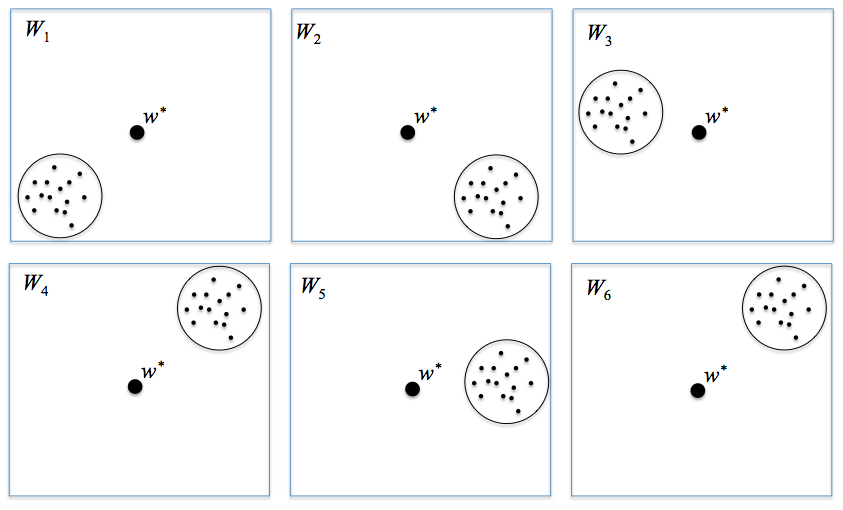
\includegraphics[width=.9\textwidth]{convexCombExample.png}
    \caption{A convex combination of $W_1,..., W_\ell$ has high min and fuzzy min-entropy, but sketching by using the component flat distributions removes all entropy.}
\label{fig:convex comb}    
\end{figure}


\section{Old Proofs}
\subsection{Flat Sources with Sketches that Write a Fixed Number of Bits}
We begin by trying to remove the restriction that every point in the metric space has a fixed number of neighbors in a distribution.  We start with sketches that write down a fixed number of bits~(independent of their input $w$).   We will show a lower bound on the number of bits that a $\sketch$ algorithm must write down.  We assume that all coins of $\sketch$ are provided to $\rec$ and that $\rec$ is deterministic~(any coins needed for $\rec$ can be flipped by $\sketch$ in this model).

\begin{lemma}
Let $W$ be a flat distribution and let $(\sketch, \rec)$ be a secure sketch for $W$.  Let $W$ be a $(c, t)$-bounded neighbor distribution.  Let $S_{coin}$ be the number of sketches that can be produced by any fixing of $coin$.  Then the error $\delta$ of $(\sketch, \rec)$ is at least $\frac{\expe_{coins}L(coins)}{c}$.  
\end{lemma}
\begin{proof}
We consider a fixed $w'$ that has $c$ neighbors in the distribution.  We assume $\rec$ has access to all coins of $\sketch$.  Furthermore, we assume that $\rec$ is deterministic and that any coins necessary are provided by $\sketch$).  

Denote by $S_{coin, R}$ the set of possible sketches for a given set of coins on all values in $R$.  Furthermore, denote by $S_{coin}$ the set of possible sketches for all values $w$~(for a given value of coin) and note that $S_{coin, R} \subset S_{coin}$.  Then $\rec(\cdot, w', coin)$ must fail to recover $|R|-|S_{coin, R}|$ fraction of $w\in R$~(recalling that $\rec$ is deterministic for this fixing of $coin$).  This means that the total number of pairs $(w, coin)$ for which $\rec$ fails to recover is $2^{|coins|}R - \sum_{coins} |S_{coin, R}|$.

This means there must exist some $w$ such that the number of $coin$ values for which $\rec$ fails to recover is 
\[
2^{|coin|} - \frac{\sum_{coin} |S_{coin, R}|}{R}.
\]
 This means that for this $w$, 
\[
\Pr_{coin}[s \leftarrow \sketch(w, coin) \wedge w = \rec(s, w', coin)] < 1- \frac{\expe |S_{coin, R}|}{|R|} = 1-\frac{\expe |S_{coin, R}|}{c} \le 1-\frac{\expe |S_{coin}| }{c}.
\]

%Consider the function $\rec(w', ss, r)$ where $ss$ is the sketch produced by $\sketch(w)$ and $r$ are the coins used by $\sketch$.  
\end{proof}

For deterministic sketches:
\[
\Hav(W|S ) = -\log \left(\sum_{s\in S} \Pr[S = s] \frac{2^{-\Hoo(W)}}{\Pr[S=s]}\right) = -\log \left(2^{-\Hoo(W)} |S| \right)  = \Hoo(W) - H_0(S).
\]

\subsection{How many bits for distribution oblivious sketch} 
\begin{lemma}
Let $\mathcal{W}$ be the set of all $t_{cor}$-well spread distributions.  Let $t = \lfloor (t_{cor}-1)/2\rfloor$ and let $(\sketch, \rec)$ be a $(\mathcal{M}, m, \tilde{m}, t )$-secure sketch.  Then the average length of $\sketch$ is at least $\log |B_{t}|$.
\end{lemma}
\bnote{what do we mean by average here?  we mean when receiving a uniform input across the coins.  Maybe, there are distributions where it writes down a little.  What's the right thing to say?  Markov?}
\begin{proof}
Let $\mathcal{M}$ be a metric space.
Let $\mathcal{W}$ be the set of all $t_{cor}$-well spread distributions on $\mathcal{M}$.  
Consider the following experiment:
\[
W\leftarrow \mathcal{W} \wedge w \leftarrow W \wedge w'\leftarrow B_{t_{cor}}(w) \wedge ss \leftarrow \sketch(w) \wedge w^* \leftarrow \rec(w', ss).
\]
That is, the adversary uniformly samples a well-spread distribution and then a point from the well-spread distribution.  
Since $(\sketch, \rec)$ works for any well-spread distribution the $\Pr[w^* = w] =1 $ in the above experiment.   Denote by $X$ the joint distribution of $w, w'$ produced in the above experiment.  Now consider the following experiment
\[
v \leftarrow U_{\mathcal{M}} \wedge v'\leftarrow B_{t_{cor}}(v) \wedge ss \leftarrow \sketch(v) \wedge v^* \leftarrow \rec(v', ss).
\]
Denote by $Y$ the joint distribution of $v, v'$ produced in the above experiment.  Then $X\overset{d}= Y$.  That is, the view of $(\sketch, \rec)$ is identically distributed in both cases.  Thus, $\Pr[v^* = v] = 1$.  For the uniform distribution the entropy retained by a secure sketch is at most $\Hav(U_{\mathcal{M}} | \sketch(U_{\mathcal{M}})) \le \log |\mathcal{M}| - \log |B_t(\cdot)|$~\cite[Lemma C.1]{DBLP:journals/siamcomp/DodisORS08}.  For a secure sketch to lose $\log |B_t(\cdot)|$ bits of entropy it must write down at least $\log |B_t(\cdot)|$ bits on average~\cite[Lemma 2.2b]{DBLP:journals/siamcomp/DodisORS08}.  Thus, $(\sketch, \rec)$ writes down at least $\log |B_t(\cdot)|$ bits on the uniform distribution and its view is identical on $X$ so it writes down at least $\log |B_{t_{cor}}|$ bits on $X$.  This completes the proof.
\end{proof}
\noindent
\textbf{Notes:} In the above lemma, the relation between the well-spreadness of the class of distributions and the correctness of the fuzzy extractor is not important and is made to match the relation in \lemref{lem:nosketchwellspread} for convenience.  The bound is purely derived from the correctness condition, the well-spreadness of the distribution can essentially be arbitrarily replaced~(as long as the maximal distance point from any point in the metric space is the same).

Furthermore, the above lemma easily extends to the setting where the distributions are not well-spread as long as there is an adversary strategy of choosing the input distribution that produces an input to sketch that is identically distributed to the uniform distribution.

The above lemma only talks about how many bits the algorithms must write down.  It does not say that the entropy of the distribution must decrease~(this is the important question).  We now proceed to this question.


\section{Examples to Consider}

\end{document}











